\section{Функциональное проектирование}

\subsection{Модуль управления пользователями}
\label{sec:user_management_functionality}

Модуль управления пользователями -- это ключевая часть системы для управления всеми учетными записями сотрудников компании и их правами доступа к различным корпоративным сервисам и ресурсам. Этот модуль позволяет администраторам централизованно управлять всеми аспектами пользовательских аккаунтов, включая создание учетных записей, назначение прав доступа и обеспечение безопасности.

\subsubsection{Cоздание пользовательских аккаунтов.} Cоздание пользовательских аккаунтов -- процесс регистрации новых сотрудников в системе. При регистрации создается учетная запись, которая включает в себя:
\begin{itemize}
    \item логин -- уникальное имя, которое пользователь будет использовать для входа в систему;
    \item пароль -- секретная комбинация символов, используемая для аутентификации пользователя;
    \item базовые права доступа, которые назначаются пользователю в зависимости от его роли в организации и задач, которые ему предстоит решать.
\end{itemize}

\subsubsection{Назначение ролей и прав доступа.} Назначение ролей и прав доступа -- после создания учетной записи пользователю назначаются определенные <<роли>>, которые могут быть связаны с его должностью или функциональной задачей в компании. Каждая роль имеет набор прав, определяющих доступ к различным сервисам и данным. Например:
\begin{itemize}
    \item администратор -- полный доступ ко всем системам и данным;
    \item менеджер -- ограниченный доступ к некоторым разделам, но возможность управлять командой;
    \item разработчик -- ограниченный доступ к некоторым разделам, но разрешена авторизация в специализированные сервисы;
    \item пользователь -- доступ только к информации, необходимой для выполнения своей работы, например, доступ только для чтения.
\end{itemize}

\subsubsection{Управление группами пользователей.} Управление группами пользователей -- пользователи могут быть объединены в группы на основе общих признаков, таких как отдел или проект. Для каждой группы настраиваются общие права доступа, что позволяет упростить управление большим количеством пользователей. Например:
\begin{itemize}
    \item группа разработчиков может иметь доступ к исходному коду, но не к финансовой отчетности;
    \item группа менеджеров проекта имеет доступ только к проектным данным и общим ресурсам, но не к конфиденциальной информации.
\end{itemize}

\subsubsection{Настройка политик безопасности.} Настройка политик безопасности -- в этом разделе администраторы могут задать обязательные требования к паролям и аутентификации:
\begin{itemize}
    \item парольная политика -- параметры, такие как минимальная длина пароля, требуемая сложность (например, наличие букв и цифр), а также правила по частоте смены пароля;
    \item двухфакторная аутентификация \textit{(2FA)} -- дополнительный уровень защиты, который требует от пользователя подтверждения своей личности через второй фактор (например, код, отправленный на телефон).
\end{itemize}

Эти меры способствуют повышению безопасности системы, предотвращая несанкционированный доступ.

\subsubsection{Централизованное управление учетными записями.} Централизованное управление учетными записями -- для повышения удобства и безопасности модуль может синхронизировать учетные записи с другими корпоративными сервисами, такими как \textit{LDAP} или \textit{Active Directory}. Это позволяет:
\begin{itemize}
    \item поддерживать единые учетные данные для всех сервисов компании;
    \item легко управлять правами доступа, поскольку все изменения выполняются в одном месте и автоматически применяются ко всем связанным сервисам.
\end{itemize}

\subsubsection{Аудит и логирование.} Аудит и логирование -- модуль фиксирует все действия пользователей, такие как:
\begin{itemize}
    \item входы и выходы из системы;
    \item изменения в настройках учетных записей, например, смену пароля или изменение прав доступа;
    \item действия, связанные с доступом к данным (например, просмотр или изменение файлов).
\end{itemize}

Эти логи могут быть использованы для анализа действий сотрудников, а также для расследования инцидентов безопасности, таких как попытки несанкционированного доступа или изменения в данных.


\subsection{Модуль мониторинга и оповещений}
\label{sec:monitoring_alerting_functionality}

Модуль мониторинга и оповещений играет ключевую роль в поддержании стабильности инфраструктуры и бесперебойной работы сервисов. Он предназначен для постоянного отслеживания состояния различных компонентов системы, анализа их работы и уведомления о любых аномалиях или сбоях. Этот модуль позволяет оперативно выявлять проблемы и минимизировать их влияние на бизнес-процессы.

\subsubsection{Сбор и анализ метрик.} Модуль регулярно собирает данные о состоянии всех ключевых компонентов системы, включая серверы, базы данных, приложения и другие устройства. Метрики, которые могут быть собраны, включают:
\begin{itemize}
    \item загрузка процессора -- измеряется в процентах, что позволяет оценить нагрузку на центральный процессор;
    \item использование памяти -- отображает, сколько оперативной памяти использует система и приложения, помогает предотвращать проблемы с нехваткой памяти;
    \item пропускная способность сети -- измеряет количество данных, которые передаются через сеть, что важно для выявления проблем с производительностью сети;
    \item состояние дисков -- отслеживается состояние жестких дисков, таких как уровень их заполненности, скорость чтения/записи и наличие ошибок;
    \item и другие параметры, такие как температура компонентов, состояние приложений, время отклика серверов и т.д.
\end{itemize}

\subsubsection{Настройка пороговых значений.} Для каждой метрики можно настроить пороговые значения, которые определяют, при каком уровне критичности или аномалии система должна отправить уведомление. Например:
\begin{itemize}
    \item если загрузка процессора превышает 90\% в течение пяти минут, то генерируется тревога;
    \item если состояние дисков приближается к 95\% заполняемости, система предупреждает о необходимости очистки дисков.
\end{itemize}

Это позволяет заранее обнаружить потенциальные проблемы и минимизировать их влияние на работу инфраструктуры.

\subsubsection{Мониторинг состояния сервисов и приложений.} Модуль осуществляет постоянное наблюдение за работоспособностью всех ключевых сервисов и приложений, таких как:
\begin{itemize}
    \item веб-серверы -- отслеживается доступность и производительность веб-приложений;
    \item базы данных -- мониторинг состояния базы данных для обнаружения сбоев или замедлений;
    \item очереди сообщений -- важный компонент для мониторинга рабочих процессов в распределенных системах;
    \item и другие критические сервисы и компоненты.
\end{itemize}

Если какой-либо сервис становится недоступен или работает с ошибками, система автоматически генерирует уведомление и отправляет его ответственным лицам.

\subsubsection{Настройка оповещений.} Система поддерживает различные способы уведомлений, что позволяет оперативно информировать ответственных сотрудников о возникших проблемах. Уведомления могут быть настроены для различных групп пользователей:
\begin{itemize}
    \item \textit{email} -- отправка уведомлений по электронной почте;
    \item \textit{Slack} -- уведомления в канал корпоративного чата;
    \item \textit{SMS} -- сообщения на мобильные устройства для уведомлений, требующих немедленного внимания;
    \item и другие каналы связи в зависимости от требований.
\end{itemize}

Уведомления могут быть настроены в зависимости от важности события: критические ошибки могут направляться техническим специалистам, а менее важные могут быть отправлены бизнес-пользователям для общего ознакомления.

\subsubsection{Интеграция с внешними системами уведомлений.} Для повышения гибкости и улучшения реакции на инциденты модуль может быть интегрирован с внешними платформами, такими как:
\begin{itemize}
    \item \textit{PagerDuty} -- система управления инцидентами и уведомлениями, которая помогает быстро реагировать на критические ситуации;
    \item \textit{Opsgenie} -- платформа для организации оповещений и управления инцидентами в крупных инфраструктурах.
\end{itemize}

Это расширяет возможности модуля и позволяет более эффективно управлять инцидентами на всех этапах их обработки.

\subsubsection{Ведение логов событий.} Модуль сохраняет все события и уведомления о состоянии системы в логах. Эти логи могут включать информацию о:
\begin{itemize}
    \item времени срабатывания уведомлений;
    \item метках тревог и порогах, которые были превышены;
    \item действиях, предпринятых для устранения инцидента;
    \item любых других значимых событиях.
\end{itemize}

Логи могут использоваться для последующего анализа, аудита и расследования инцидентов, что помогает улучшать процессы мониторинга и предотвращать повторные сбои.

\subsection{Модуль хранилища секретов}
\label{sec:secrets_storage_functionality}

Модуль хранилища секретов отвечает за безопасное хранение и управление конфиденциальной информацией, такой как ключи, пароли, сертификаты и другие чувствительные данные. Основной функционал модуля включает:

\begin{itemize}
    \item безопасное хранение секретов -- секреты (пароли, ключи и сертификаты) хранятся в зашифрованном виде, и доступ к ним осуществляется через защищенные каналы; 
    \item централизованный доступ к секретам -- все сервисы и пользователи получают доступ к секретам через централизованный хранилище, что упрощает управление и повышает безопасность; 
    \item настройка политик доступа -- можно настраивать, какие пользователи или группы пользователей могут иметь доступ к конкретным секретам, политики могут учитывать уровни доступа и типы секретов (например, доступ к базе данных или \textit{API}-ключам); 
    \item ротация секретов -- автоматическая ротация ключей и паролей для повышения безопасности, это может происходить по расписанию или по запросу; 
    \item интеграция с другими модулями -- хранилище секретов интегрируется с другими компонентами инфраструктуры, такими как системы оркестрации контейнеров или виртуальных машин, для автоматического использования секретов; 
    \item ведение логов доступа -- все операции с секретами, включая их доступ, изменения и ротацию, логируются для обеспечения аудита. 
\end{itemize}

\subsection{\textit{Kubernetes} кластер}
\label{sec:kubernetes_cluster_functionality}

Модуль \textit{Kubernetes} кластеров предоставляет возможности для оркестрации контейнеризированных приложений, автоматизации их развертывания, масштабирования и обеспечения высокой доступности. Основной функционал модуля направлен на управление жизненным циклом приложений в контейнерах, что включает автоматическое развертывание, масштабирование, мониторинг и восстановление. Этот модуль также помогает улучшить производительность и отказоустойчивость инфраструктуры, предоставляя гибкие инструменты для работы с контейнерами. Диаграмма компонентов \textit{Kubernetes} представлена на рисунке \ref{fig:kubernetes_cluster_functionality:k8s_components}.
\begin{figure}[ht]
    \centering
    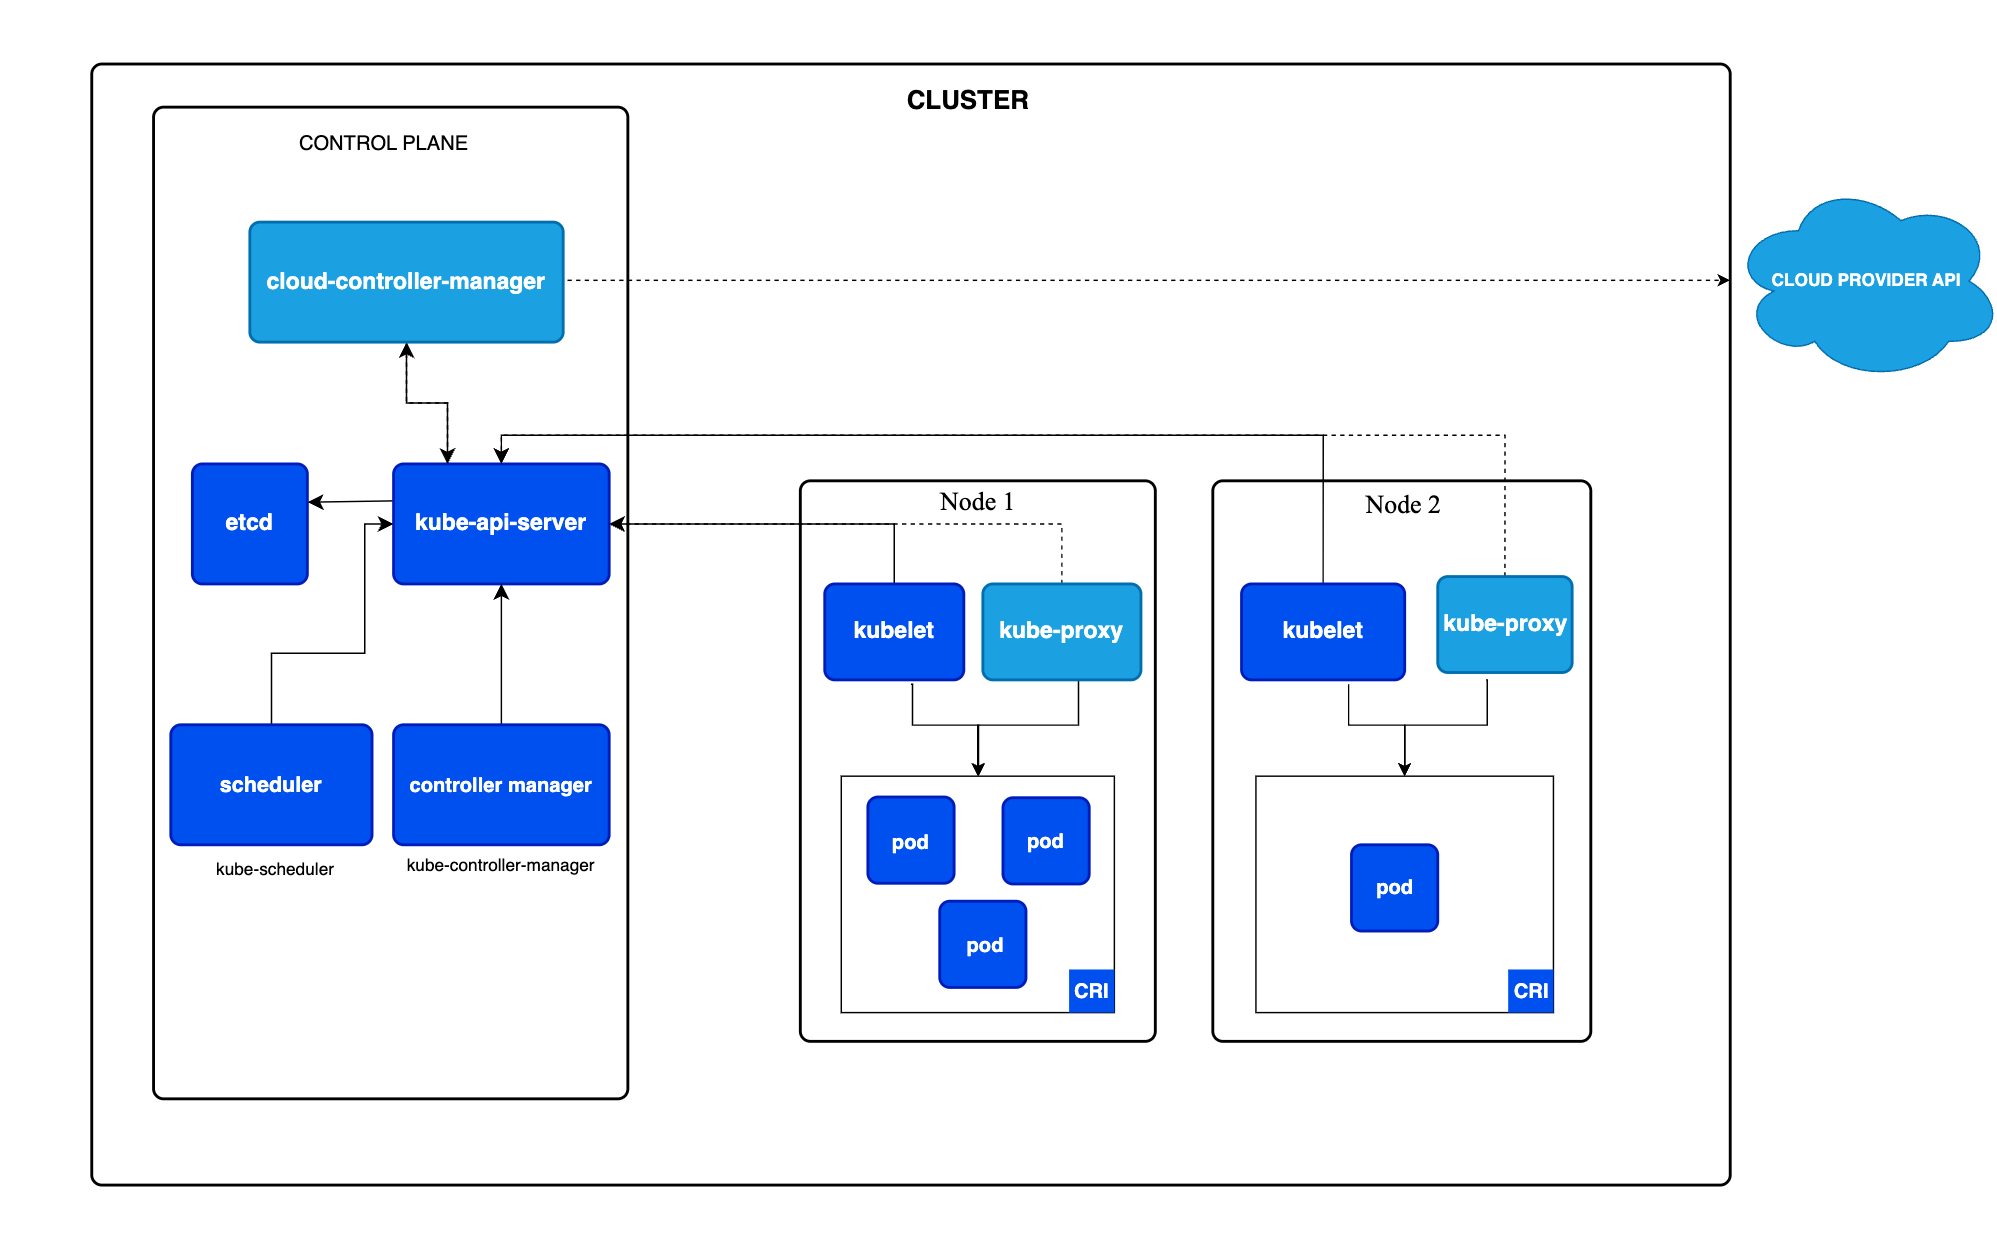
\includegraphics[width=0.75\linewidth]{\commonSecPathPrefix/../img/kubernetes-cluster-architecture.png}
    \caption{Диаграмма компонентов \textit{k8s}}
    \label{fig:kubernetes_cluster_functionality:k8s_components}
\end{figure}

Основной функционал модуля:

\begin{enumerate}
    \item Автоматическое развертывание контейнеров -- \textit{Kubernetes} позволяет автоматически развертывать контейнеризованные приложения, используя конфигурационные файлы в формате \textit{YAML}, которые описывают параметры приложений, такие как количество реплик, настройки ресурсов, переменные окружения и зависимости. \textit{Kubernetes} управляет жизненным циклом приложений, начиная от их развертывания и заканчивая удалением или обновлением.
    \item Масштабирование приложений -- модуль поддерживает как вертикальное, так и горизонтальное масштабирование приложений, что позволяет адаптировать инфраструктуру под изменяющиеся нагрузки. \textit{Kubernetes} автоматически увеличивает или уменьшает количество реплик приложения в зависимости от текущей нагрузки или в ответ на изменения в метриках, таких как загрузка процессора, использование памяти или количество запросов.
    \item Автоматическое восстановление сервисов -- в случае сбоя контейнера или приложения \textit{Kubernetes} автоматически перезапускает контейнеры или перераспределяет их на другие узлы, обеспечивая минимальное время простоя. Это особенно важно для обеспечения бесперебойной работы приложений и минимизации влияния сбоев на пользователей.
    \item Управление сетью и хранилищем данных -- \textit{Kubernetes} управляет сетевыми ресурсами, создавая виртуальные сети для обеспечения связи между контейнерами и сервисами. Он также автоматизирует подключение и управление хранилищами данных, такими как \textit{Persistent Volumes}, которые могут быть использованы контейнерами для хранения данных, сохраняя их даже в случае перезапуска контейнера.
    \item Мониторинг ресурсов кластера -- \textit{Kubernetes} предоставляет подробную информацию о состоянии всех компонентов кластера, таких как использование процессора, памяти, дисков, сети и других ресурсов. Метрики о состоянии кластера и его компонентов помогают оперативно принимать решения о масштабировании или перераспределении нагрузки, а также следить за эффективностью использования ресурсов.
    \item Репликация и разделение нагрузки -- для повышения отказоустойчивости и производительности \textit{Kubernetes} обеспечивает автоматическое разделение нагрузки между несколькими репликами приложений. Это гарантирует, что приложение будет продолжать работать, даже если один из экземпляров выйдет из строя, и позволяет равномерно распределять трафик между всеми доступными репликами.
    \item Интеграция с \textit{CI/CD} -- модуль \textit{Kubernetes} поддерживает интеграцию с инструментами непрерывной интеграции и доставки (например, \textit{Jenkins}, \textit{GitLab CI}), что позволяет автоматизировать процесс развертывания новых версий приложений. Это позволяет оперативно обновлять приложения с минимальными рисками и простоями, а также ускоряет процесс выпуска новых функций и исправлений.
    \item Управление конфигурацией и секретами -- \textit{Kubernetes} предоставляет механизмы для безопасного хранения конфигураций приложений и секретных данных, таких как пароли, ключи и токены, с использованием \textit{ConfigMaps} и \textit{Secrets}. Эти механизмы позволяют централизованно управлять конфигурациями, обеспечивая безопасность и соблюдение стандартов при развертывании приложений.
    \item Интеграция с системами наблюдения -- \textit{Kubernetes} легко интегрируется с различными системами мониторинга, такими как \textit{Prometheus}, для сбора и анализа метрик, что позволяет отслеживать работу приложений и кластера в реальном времени. Эти данные могут быть использованы для дальнейшего анализа и принятия решений по оптимизации и улучшению инфраструктуры.
\end{enumerate}

\subsection{Модуль работы с облачной инфраструктурой}
\label{sec:cloud_infrastructure_functionality}

Модуль работы с облачной инфраструктурой предназначен для управления виртуальными ресурсами, такими как виртуальные машины, сети и хранилища, в облачной среде. Основной функционал модуля включает:

\begin{itemize}
    \item создание и управление виртуальными машинами -- модуль позволяет создавать виртуальные машины в облаке, управлять их конфигурациями, масштабировать и удалять; 
    \item настройка сетей и хранилища -- управление виртуальными сетями и хранилищем данных, включая настройку \textit{VPN} и \textit{firewall} правил, а также создание дисков и бакетов; 
    \item масштабирование ресурсов -- автоматическое или ручное масштабирование виртуальных машин и других сервисов в зависимости от требований нагрузки; 
    \item \textit{IaC (Infrastructure as Code)} -- использование описания инфраструктуры в виде кода (\textit{Terraform}, \textit{CloudFormation}) для автоматизированного создания, управления и удаления ресурсов; 
    \item интеграция с другими сервисами -- взаимодействие с другими сервисами облачной инфраструктуры, такими как базы данных, сервисы для хранения больших данных и т.д.; 
    \item управление безопасностью и доступом -- настройка прав доступа и безопасность виртуальных машин и других сервисов облака, включая использование \textit{IAM} ролей и политик. 
\end{itemize}

\subsection{Модуль управления доступом через \textit{VPN}}
\label{sec:vpn_access_functionality}

Модуль управления доступом через \textit{VPN} позволяет безопасно подключать сотрудников к корпоративной сети удаленно. Основной функционал модуля включает:

\begin{itemize}
    \item создание \textit{VPN}-сессий -- создание защищенных подключений для сотрудников, работающих удаленно, для этого используются современные протоколы шифрования и аутентификации; 
    \item настройка шифрования и протоколов безопасности -- настройка протоколов безопасности для защиты трафика, таких как \textit{IPsec}, \textit{SSL/TLS}; 
    \item политики доступа для пользователей -- настройка прав доступа для разных категорий пользователей, например, ограничения на доступ к определенным ресурсам в сети; 
    \item двухфакторная аутентификация -- интеграция с системами двухфакторной аутентификации (например, через мобильные приложения или \textit{SMS}); 
    \item мониторинг \textit{VPN}-сессий -- мониторинг активных подключений, времени сеансов и использования ресурсов; 
    \item ведение логов подключений -- сохранение всех подключений и действий, выполненных пользователями в сети, для последующего анализа и аудита. 
\end{itemize}

\subsection{Модуль автоматизации с помощью \textit{GitOps}}
\label{sec:gitops_automation_functionality}

Модуль автоматизации с помощью \textit{GitOps} предоставляет возможности для автоматического развертывания, управления инфраструктурой и приложениями через \textit{Git} репозитории, что позволяет обеспечить прозрачность, повторяемость и контроль версий. Вся инфраструктура и конфигурации хранятся в репозиториях, а изменения управляются через \textit{Git} с использованием принципов DevOps. 

Диаграмма компонентов \textit{Flux CD} представлена на рисунке \ref{fig:gitops_automation_functionality:fluxcd.png}.
\begin{figure}[ht]
    \centering
    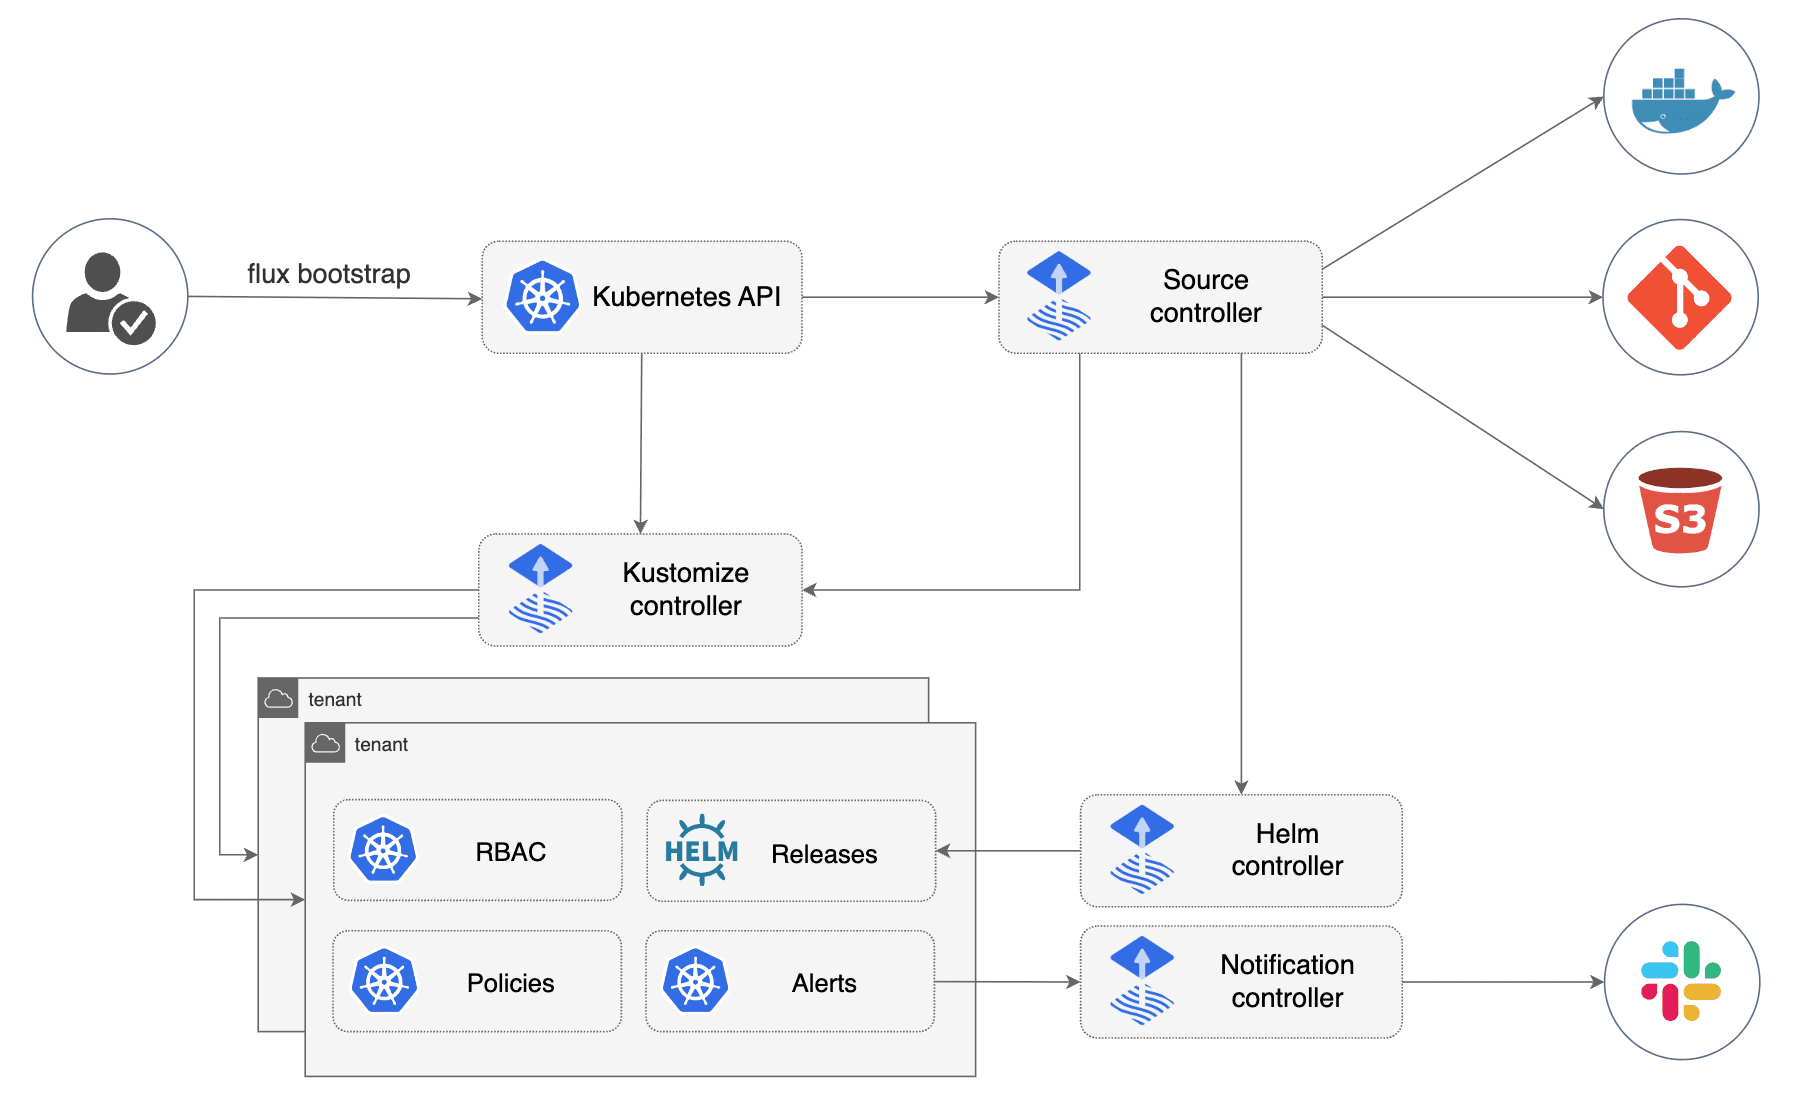
\includegraphics[width=0.85\linewidth]{\commonSecPathPrefix/../img/fluxcd.png}
    \caption{Диаграмма компонентов \textit{Flux CD}}
    \label{fig:gitops_automation_functionality:fluxcd.png}
\end{figure}

Этот подход минимизирует ошибки, улучшает контроль и ускоряет процесс обновления инфраструктуры, благодаря автоматизации процессов, уменьшению человеческого вмешательства и обеспечению согласованности между различными средами, что способствует повышению надежности и безопасности системы в целом.
Основной функционал модуля:

\begin{enumerate}
    \item Автоматизированное развертывание через \textit{Git} -- автоматическое развертывание инфраструктуры и приложений, используя конфигурации, хранящиеся в \textit{Git} репозиториях. Каждый раз при внесении изменений в репозиторий автоматически инициируется процесс развертывания, что минимизирует человеческие ошибки и ускоряет процесс внедрения новых версий.
    \item \textit{CI/CD} процессы -- интеграция с системами непрерывной интеграции и доставки (например, \textit{Jenkins}, \textit{GitLab CI}, \textit{CircleCI}), что позволяет автоматизировать развертывание и обновление приложений и инфраструктуры. Каждый коммит в репозиторий может триггерить автоматические тесты, сборки и развертывание, обеспечивая постоянный контроль качества и актуальность версий.
    \item Мониторинг состояния приложений -- мониторинг развернутых приложений и инфраструктуры через \textit{GitOps}. Система отслеживает текущее состояние приложений и сервисов, чтобы обеспечить соответствие фактического состояния заданному описанию в репозиториях. В случае отклонений или проблем автоматически отправляются уведомления, а также предоставляется возможность откатить изменения, чтобы восстановить стабильное состояние.
    \item Управление конфигурациями через \textit{Git} -- все конфигурации, включая описание инфраструктуры, параметры развертывания, настройки приложений, хранятся в \textit{Git} репозиториях, что обеспечивает версионность и прозрачность изменений. Это позволяет удобно отслеживать, какие изменения были сделаны, кто их сделал, и когда, обеспечивая аудит и контроль над всеми изменениями в инфраструктуре.
    \item Интеграция с другими модулями -- модуль \textit{GitOps} интегрируется с другими модулями инфраструктуры для обеспечения консистентности и безопасности развертываемых приложений. Например, он может работать в связке с модулями мониторинга, безопасности, управления пользователями, что позволяет обеспечить комплексный подход к автоматизации управления инфраструктурой и приложениям.
    \item Автоматическое откатывание изменений -- если при развертывании новой версии приложения или изменения в инфраструктуре произошел сбой или возникли проблемы, модуль \textit{GitOps} может автоматически откатить изменения, возвращая инфраструктуру в стабильное состояние, описанное в репозитории. Это обеспечивает высокий уровень отказоустойчивости и минимизирует возможное время простоя в случае проблем с новой версией.
    \item Управление секретами через \textit{GitOps} -- безопасное хранение и управление секретами, такими как ключи \textit{API}, пароли и сертификаты, с помощью интеграции с хранилищами секретов (например, \textit{HashiCorp Vault}, \textit{Kubernetes Secrets}) и автоматическое обновление их конфигурации при изменении значений в репозиториях, обеспечивая безопасность и управление доступом к чувствительным данным.
    \item Интеграция с системами контроля версий и тестирования -- использование \textit{Git} как единого источника правды для конфигураций и изменений в инфраструктуре дает возможность интегрировать систему с процессами тестирования и контроля качества, что позволяет обеспечить качество и стабильность развертываемых приложений на всех этапах разработки и эксплуатации.
    \item Отслеживание состояния через \textit{GitOps dashboard} -- централизованный интерфейс (например, \textit{ArgoCD}, \textit{Flux}) позволяет отслеживать статус всех развернутых приложений, их текущие конфигурации и любые отклонения от желаемого состояния. Это дает визуальное представление о текущем состоянии инфраструктуры и упрощает управление и принятие решений о необходимых изменениях.
\end{enumerate}

В результате, использование модуля \textit{GitOps} способствует значительному улучшению процессов управления инфраструктурой и приложениями, обеспечивая не только высокую степень автоматизации и надежности, но и улучшенную видимость всех изменений. Это позволяет ускорить процессы разработки и доставки, уменьшить риски ошибок, а также повысить безопасность и контроль над всеми аспектами инфраструктуры. Благодаря интеграции с различными инструментами и системами, подход \textit{GitOps} предлагает гибкость и масштабируемость, соответствующие требованиям современного подхода к разработке и эксплуатации программных решений.